\documentclass[a4paper,12pt]{report}
\usepackage{alltt, fancyvrb, url}
\usepackage{graphicx}
\usepackage[utf8]{inputenc}
\usepackage{float}
\usepackage{hyperref}
\usepackage{csquotes}
\usepackage{listings}
% Questo commentalo se vuoi scrivere in inglese.
\usepackage[italian]{babel}
\usepackage[italian]{cleveref}
\usepackage{xurl}

\lstdefinestyle{json}{
  basicstyle=\ttfamily\small,
  columns=fullflexible,
  showstringspaces=false,
  commentstyle=\color{gray}\upshape
}

\title{%
  IoT Assignment 3 \\
  \large Smart Room}

\author{Mattia Panni \\ Riccardo Fiorani \\ Eleonora Falconi \\ Alesja Delja}
\date{\today}

\begin{document}
\maketitle
\tableofcontents


\chapter{Design}
In questa sezione verranno spiegate le scelte di design intraprese, in una prima fase di interazione fra i membri del gruppo, e che ci hanno permesso, dopo una raffinazione successiva, di arrivare alla soluzione finale del sistema.
\section{Architettura}
Come da specifiche, tutto il progetto è stato fin da subito suddiviso nei cinque sottosistemi 
\begin{enumerate}
    \item \emph{Room Sensor-Board} (ESP)
    \item \emph{Room Service} (backend, PC)
    \item \emph{Room Dashboard} (frontend, PC)
    \item \emph{Room Mobile App} (android)
    \item \emph{Room Controller} (arduino)
\end{enumerate}

Di seguito sono riportate le scelte progettuali per le parti più critiche.
\subsection{Room Controller (Arduino)}
Per il sottosistema imputato al controllo della luce e delle tende, sono state concepite due macchine a stati finiti che descrivessero il comportamento di ciascuno di questi due componenti. Si è inoltre pensato di fare in modo che entrambe fossero \textbf{asincrone}, ovvero che non dipendessero dalla frequenza di clock, ma unicamente dagli eventi che si verificano all'interno della stanza. In particolare si ha
\begin{enumerate}
    \item \textbf{Smart Lightining Subsystem}. Sistema di controllo per la luce interna alla casa. Come da specifiche, esso potrà essere sia pilotato manualmente da uno fra app android e dashboard, che lasciato autonomo. Nel primo caso, sarà possibile scegliere se accendere o spegnere la luce, indipendentemente dal livello di luce e movimento all'interno della stanza. Nel secondo caso, invece, qualora ci sia movimento e la stanza fosse buia, la luce verrebbe accesa. Qualora, invece, non vi fosse nessuno all'interno, la luce si spegnerebbe.
    \item \textbf{Smart Roller Blinds System}. Sistema che controlli il livello di apertura delle tende. Se posto in automatico, al primo movimento registrato all'interno della stanza dopo le 8 del mattino le tende dovranno aprirsi. Viceversa, in assenza di movimento dalle 19 in poi, le tende dovranno chiudersi. Invece se posto in manuale, sarà l'utente, mediante app per dispositivo mobile o interfaccia web, a decidere se tenerle chiuse o aprirle.
\end{enumerate}

In seguito a una prima discussione fra i membri del gruppo è anche sorta l'ipotesi di modellare il sistema in maniera differente, affinché sia luce che tende potessero essere integrate in un unico diagramma. Come si vedrà in seguito, infatti, in entrambi i casi abbiamo due macro stati (\emph{Automatic} e \emph{Manual}). L'ipotesi era quella di sfruttare la sintassi UML della decomposizione ortogonale (AND). In particolare per i due macrostati automatico e manuale, si è pensato di costruire più corsie parallele al loro interno, una per la luce, e l'altra per le tende. Tuttavia abbiamo preferito non intraprendere questa strada perché volevamo fornire maggiore libertà agli utenti. In particolare, qualora si entrasse nello stato manuale utilizzando questo design, sia tende che luce si sarebbero dovute controllare manualmente. Se invece si tengono separate è possibile decidere di controllare una sola delle due cose. 
\subsubsection{Smart Lightning Subsystem}
La macchina a stati finiti pensata per questo macro sistema è rappresentata in figura \ref{fig:FSMSmartLightning}.

Il diagramma, come già anticipato, si compone di due macro stati 
\begin{itemize}
    \item \textbf{Automatic}. Rappresenta lo stato in cui la luce si gestisce autonomamente. Ovviamente all'interno di questo stato avremo i due stati relativi allo stato di accensione o spegnimento della luce. In particolare 
    \begin{itemize}
        \item \textbf{On}. Luce accesa.
        \item \textbf{Off}. Luce spenta.
    \end{itemize}
    Per passare da On a Off sarà necessario che all'interno della stanza non si rilevi più la presenza di alcun individuo (in figura indicato con \textbf{!M} (Not Motion)). Viceversa, sarà possibile spostarsi da Off a On qualora si rilevi movimento e la stanza fosse buia (In figura \textbf{M} (Motion) e condizione di guardia \textbf{[Dark]}). 
    \item \textbf{Manual}. Lo stato in cui la lampada è comandata manualmente. Essa conterrà due sottostati 
    \begin{itemize}
        \item \textbf{On'}
        \item \textbf{Off'}
    \end{itemize}
    I quali, sebbene aventi nomi differenti dagli stati di ``Automatic'' per esigenze di sintassi UML, si comportano in maniera identica. 
    Ciò che cambia è la modalità di transizione da un sottostato all'altro che avviene a seguito dell'azione di un utente.
\end{itemize}

\begin{figure}[H]
\centering
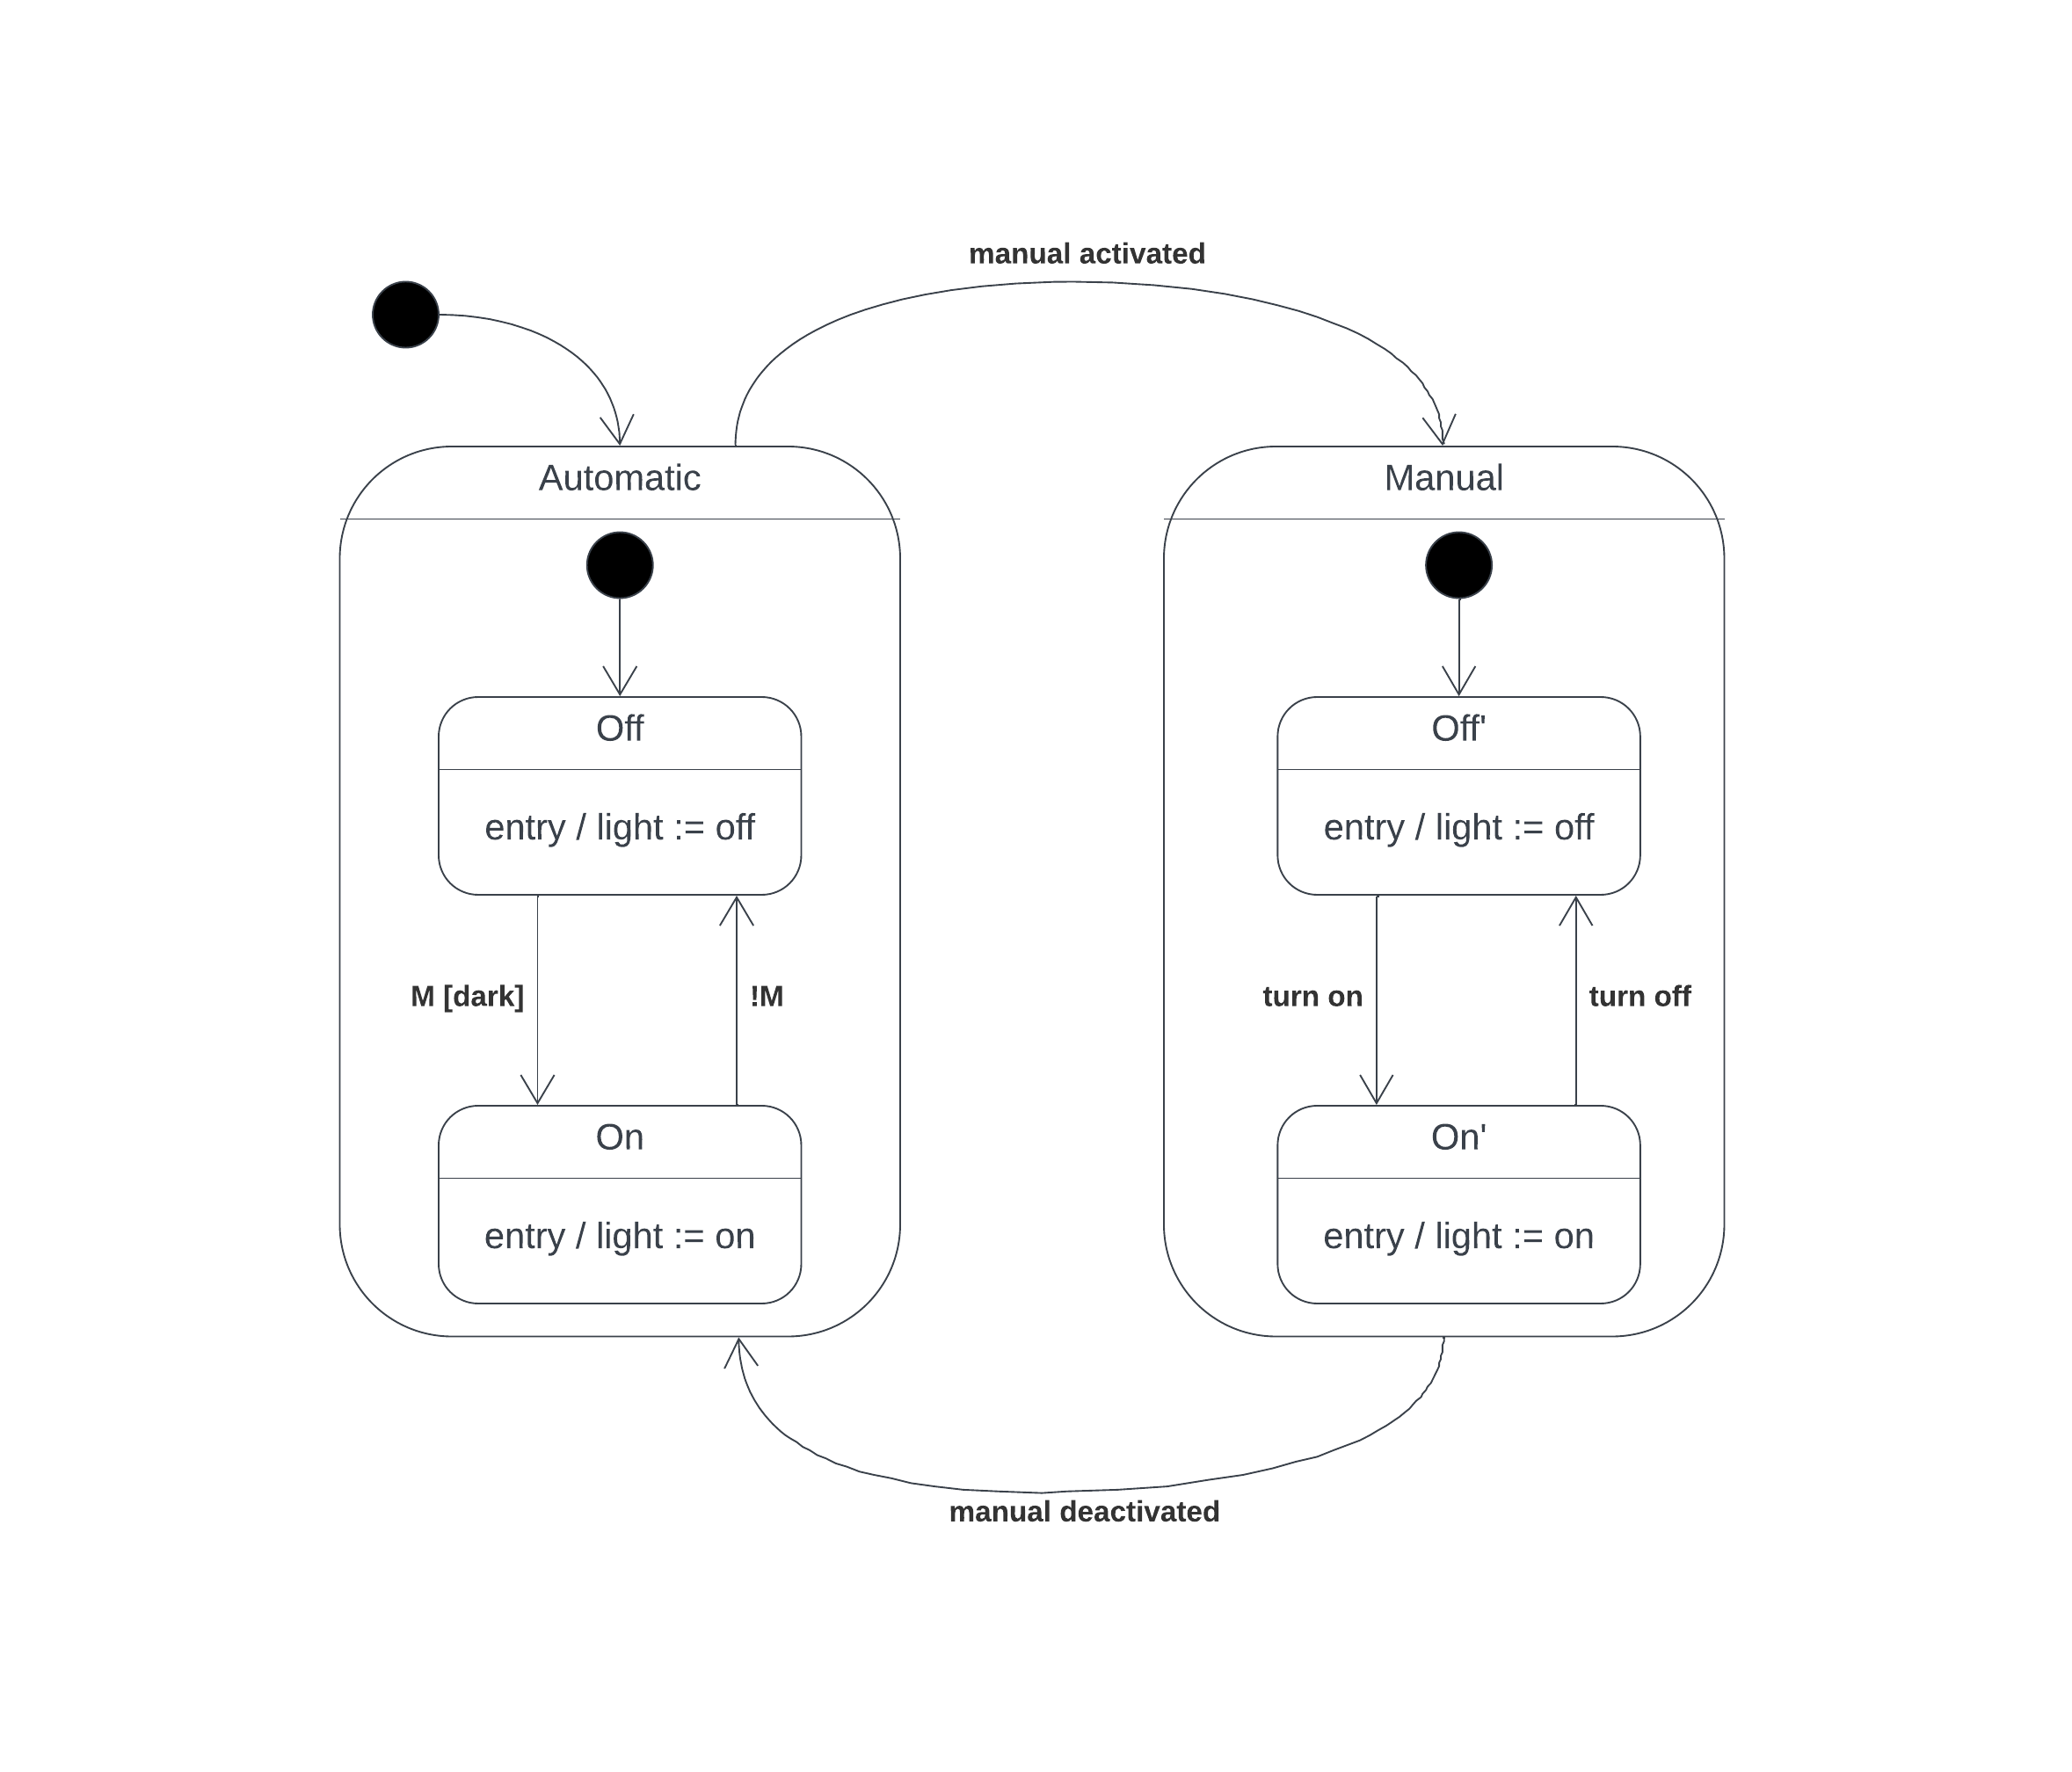
\includegraphics[width=\textwidth]{img/State - Light.png}
\caption{Smart Lightning System Finite State Machine.}
\label{fig:FSMSmartLightning}
\end{figure}


\subsubsection{Smart Roller Blinds System}
Come mostra la figura \ref{fig:FSMSmartBlinds}, analogamente all FSM relativa alla lampada, il diagramma si suddivide in due macrostati
\begin{enumerate}
    \item \textbf{Automatic}. In questo stato il sistema è completamente autonomo. In particolare le transizioni fra i due stati interni 
    \begin{itemize}
        \item \textbf{Fully Unrolled}. La tenda è completamente chiusa, in altre parole ha un angolo di  chiusura posto al 100\%. 
        \item \textbf{Fully Rolled}. Completamente aperta, 0\%.
    \end{itemize}
    avvengono, da unrolled a rolled qualora si rilevasse un movimento in un orario compreso fra le 8:00 e le 18:59, mentre il viceversa qualora non si rilevasse più movimento e l'ora fosse fra le 19:00 e le 7:59.
    \item \textbf{Manual}. In questo stato, indipendentemente dall'ora del giorno e del movimento registrato nella stanza, le tende potranno essere aperte o chiuse dall'utente che possiede il controllo (tramite app o web page). In questo caso si è optato per definire un unico sotto stato \textbf{Rolled}, che, a differenza di fully rolled e fully unrolled, avrà un angolo di apertura pari a $X$ (variabile definita nell'intervallo $[0, 100\%]$) che, come mostra il post-it in figura, andrà mappata internamente nel range di apertura delle tende (nell'intervallo $[0, 1023]$). Per cambiare l'apertura delle tende nel macro stato manuale si dovrà invocare un metodo ``update(X)'' il cui parametro corrisponde al grado di apertura delle tende.
\end{enumerate}
Le transizioni fra i macro stati avvengono qualora si attivi (o disattivi) la modalità manuale.

\begin{figure}[H]
\centering
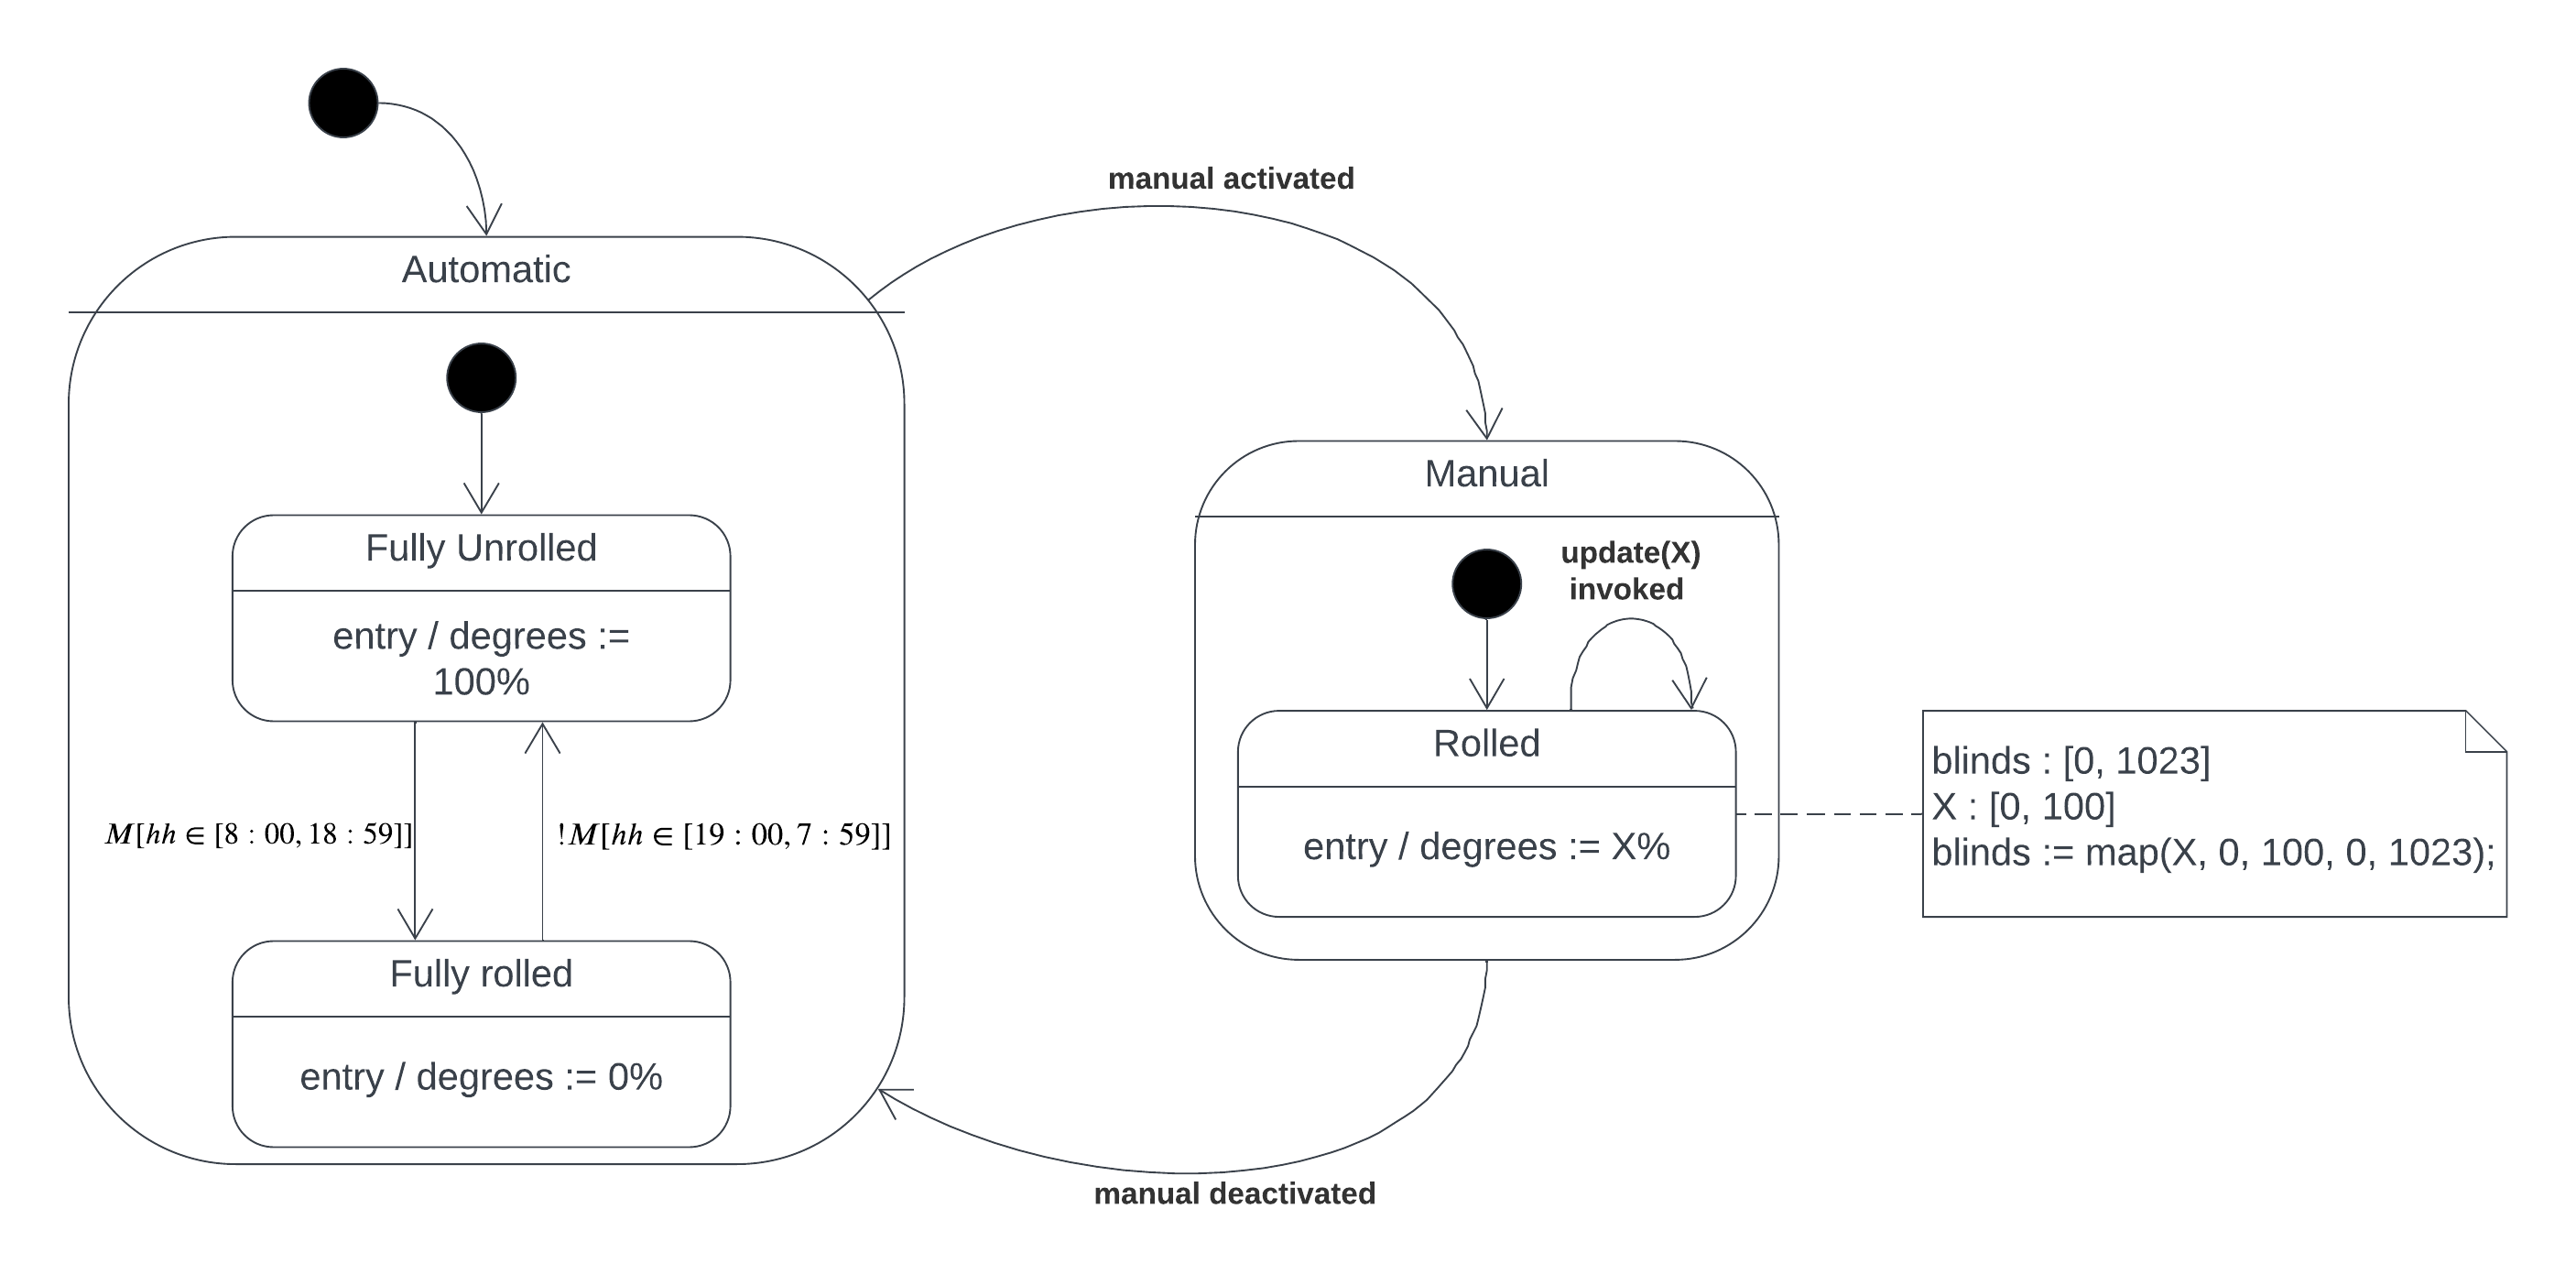
\includegraphics[width=\textwidth]{img/State - roller blinds.png}
\caption{Smart Roller Blinds System Finite State Machine.}
\label{fig:FSMSmartBlinds}
\end{figure}




\section{Architettura nel dettaglio}
In questo paragrafo si spiegherà nel dettaglio l'architettura implementata.
Poiché il sistema è suddiviso in cinque sottosistemi, ciascuno considerabile indipendente dal resto, tratteremo ciascuno di essi singolarmente.

\subsection{Room Sensor Board (ESP)}
Come già anticipato, il compito dell'ESP32 è quello di inviare periodicamente i dati registrati dalla fotoresistenza e dal sensore di movimento (PIR) a un server remoto tramite WiFi, utilizzando il protocollo MQTT.

L'architettura del sistema è rappresentata in figura \ref{fig:espclassi}

\begin{figure}[H]
    \centering
    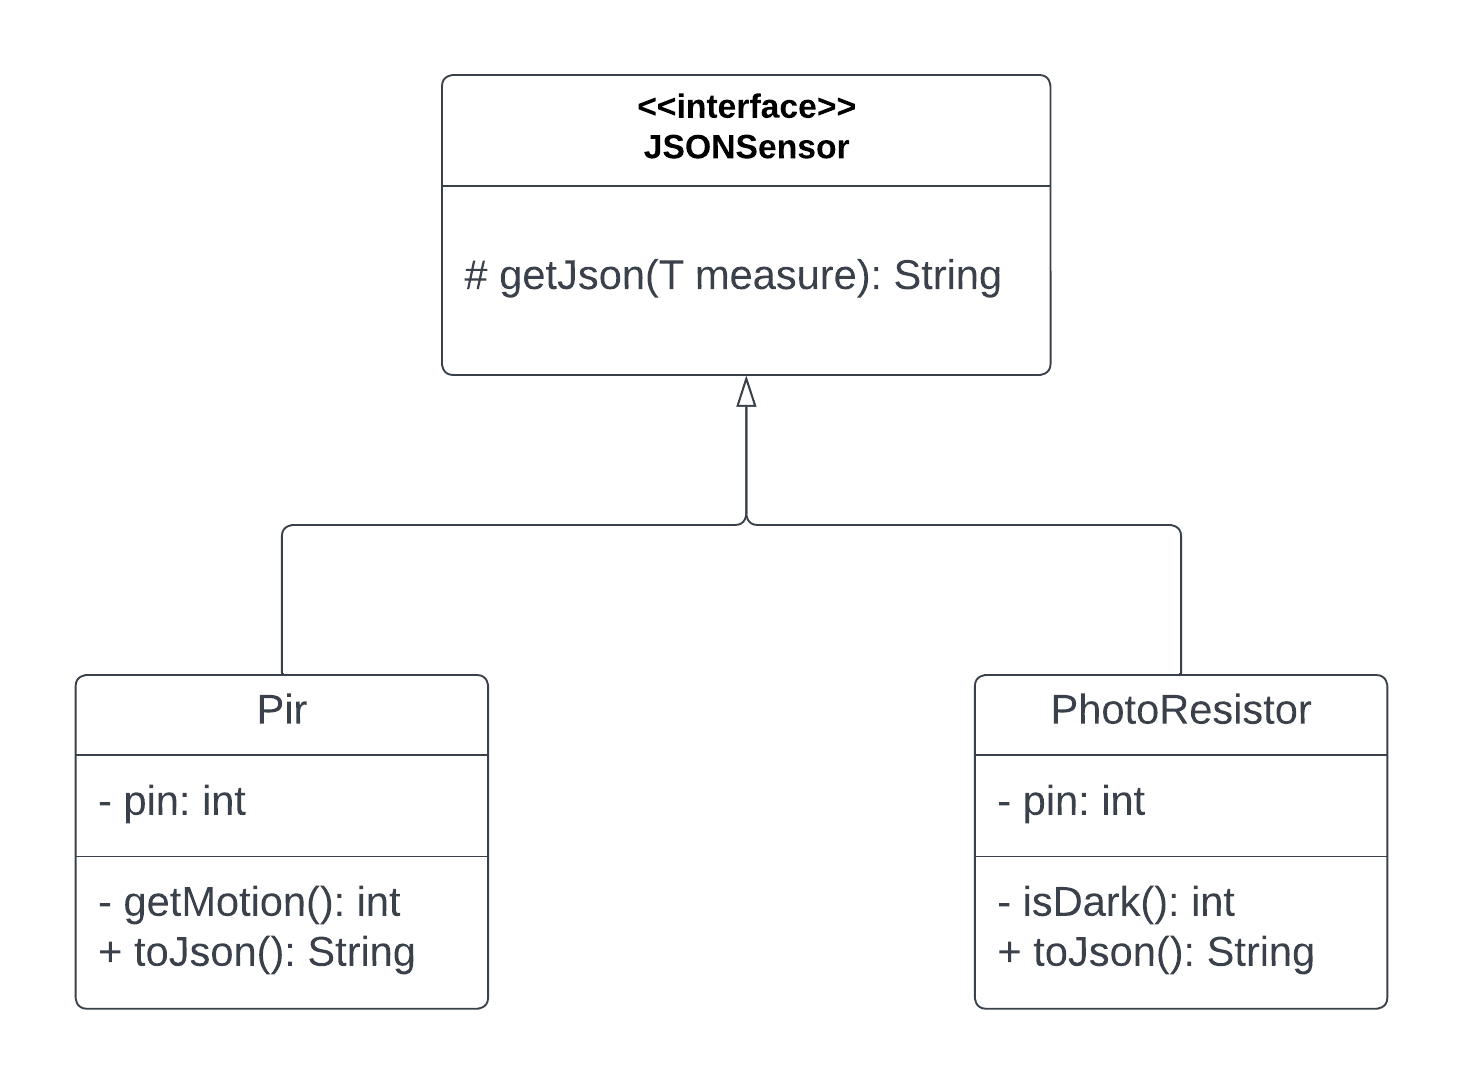
\includegraphics[width=0.7\textwidth]{img/Classi - esp.png}
    \caption{Diagramma delle classi sistema Room Sensor Board.}
    \label{fig:espclassi}
\end{figure}

Poiché è necessario comunicare al server le seguenti informazioni
\begin{itemize}
    \item \emph{Sensore}. Occorre indicare al server da quale sensore (pir o fotoresistenza) proviene la misurazione.
    \item \emph{Misura}. Rappresenta il valore rilevato dal sensore in un dato istante.
    \item \emph{Timestamp}. Utilizzato per tenere traccia dell'istante in cui la misurazione è stata effettuata.
\end{itemize}

abbiamo deciso di strutturare tutti i messaggi inviati al server nel seguente formato JSON
\begin{lstlisting}[style=json]
{
  "sensor": "pir_sensor/photo_resistor",
  "measure": 0/1,
  "timestamp": 1688505106
}
\end{lstlisting}
Per fare questo abbiamo definito un'interfaccia comune ai due sensori, chiamata \texttt{JSONSensor} che incorpora la logica necessaria per creare una stringa JSON avente la struttura desiderata. Poiché i tipi di misurazione possono essere diversi a seconda del sensore che implementa questa interfaccia, è stato utilizzato un parametro di template $T$.

A questo punto, all'interno del file .ino, abbiamo istanziato un oggetto \texttt{Adafruit\_MQTT\_Client} dell'omonima libreria. Questo oggetto è stato iscritto ai topic MQTT ``topic\_light'' e ``topic\_motion'', corrispondenti ai rispettivi sensori.
All'interno del \texttt{loop()} vengono pubblicate sui rispettivi topic le misurazioni effettuate dai sensori, con cadenza di un secondo.

\subsection{Room Service (Backend)}
Il sottosistema è suddiviso in diversi componenti autonomi che offrono ciascuno un particolare servizio.
Per la comunicazione con Arduino, è presente una classe definita \texttt{SerialService} che si occupa di mantenere attivo un canale di comunicazione seriale. 
Per quanto riguarda l'interazione con il frontend (la dashboard html) è stato implementato un \texttt{AbstractVerticle} della libreria \texttt{Vertx} all'interno della classe \texttt{HTTPService}. Poiché l'interazione dev'essere bidirezionale, ovvero il server deve inviare dati al frontend e viceversa, 
abbiamo deciso di utilizzare il protocollo \texttt{WebSocket}, che permette di mantenere una connessione persistente fra client e server.
La prima implementazione del sottosistema prevedeva l'utilizzo di chiamate axios da parte di javascript per inviare richieste HTTP al server con frequenza di un secondo (con \texttt{setInterval()}), ma ci siamo resi conto che questo approccio non era adatto al nostro caso d'uso, poiché le richieste HTTP sono state progettate per essere stateless, ovvero non mantengono alcuno stato fra una richiesta e l'altra. Questo significa che, affinché il server invii dati al client, il client deve inviare una richiesta HTTP per riceverli, ma questo comporta un overhead di comunicazione non necessario, poiché il client deve inviare una richiesta per ricevere dati che il server ha già pronti. Per questo motivo abbiamo deciso di utilizzare il protocollo WebSocket, che permette di mantenere una connessione persistente fra client e server, in modo che il server possa inviare dati al client in qualsiasi momento, senza che il client debba inviare una richiesta.

Per quanto riguarda la comunicazione con l'ESP32, abbiamo utilizzato il protocollo MQTT, che permette di inviare messaggi a un topic, che può essere iscritto da uno o più client. In questo modo, non appena l'ESP invia un messaggio ad uno dei due topic, il server lo riceve immediatamente.

Di seguito è riportato un diagramma delle classi che spiega l'interazione fra le parti
\begin{figure}[H]
    \centering
    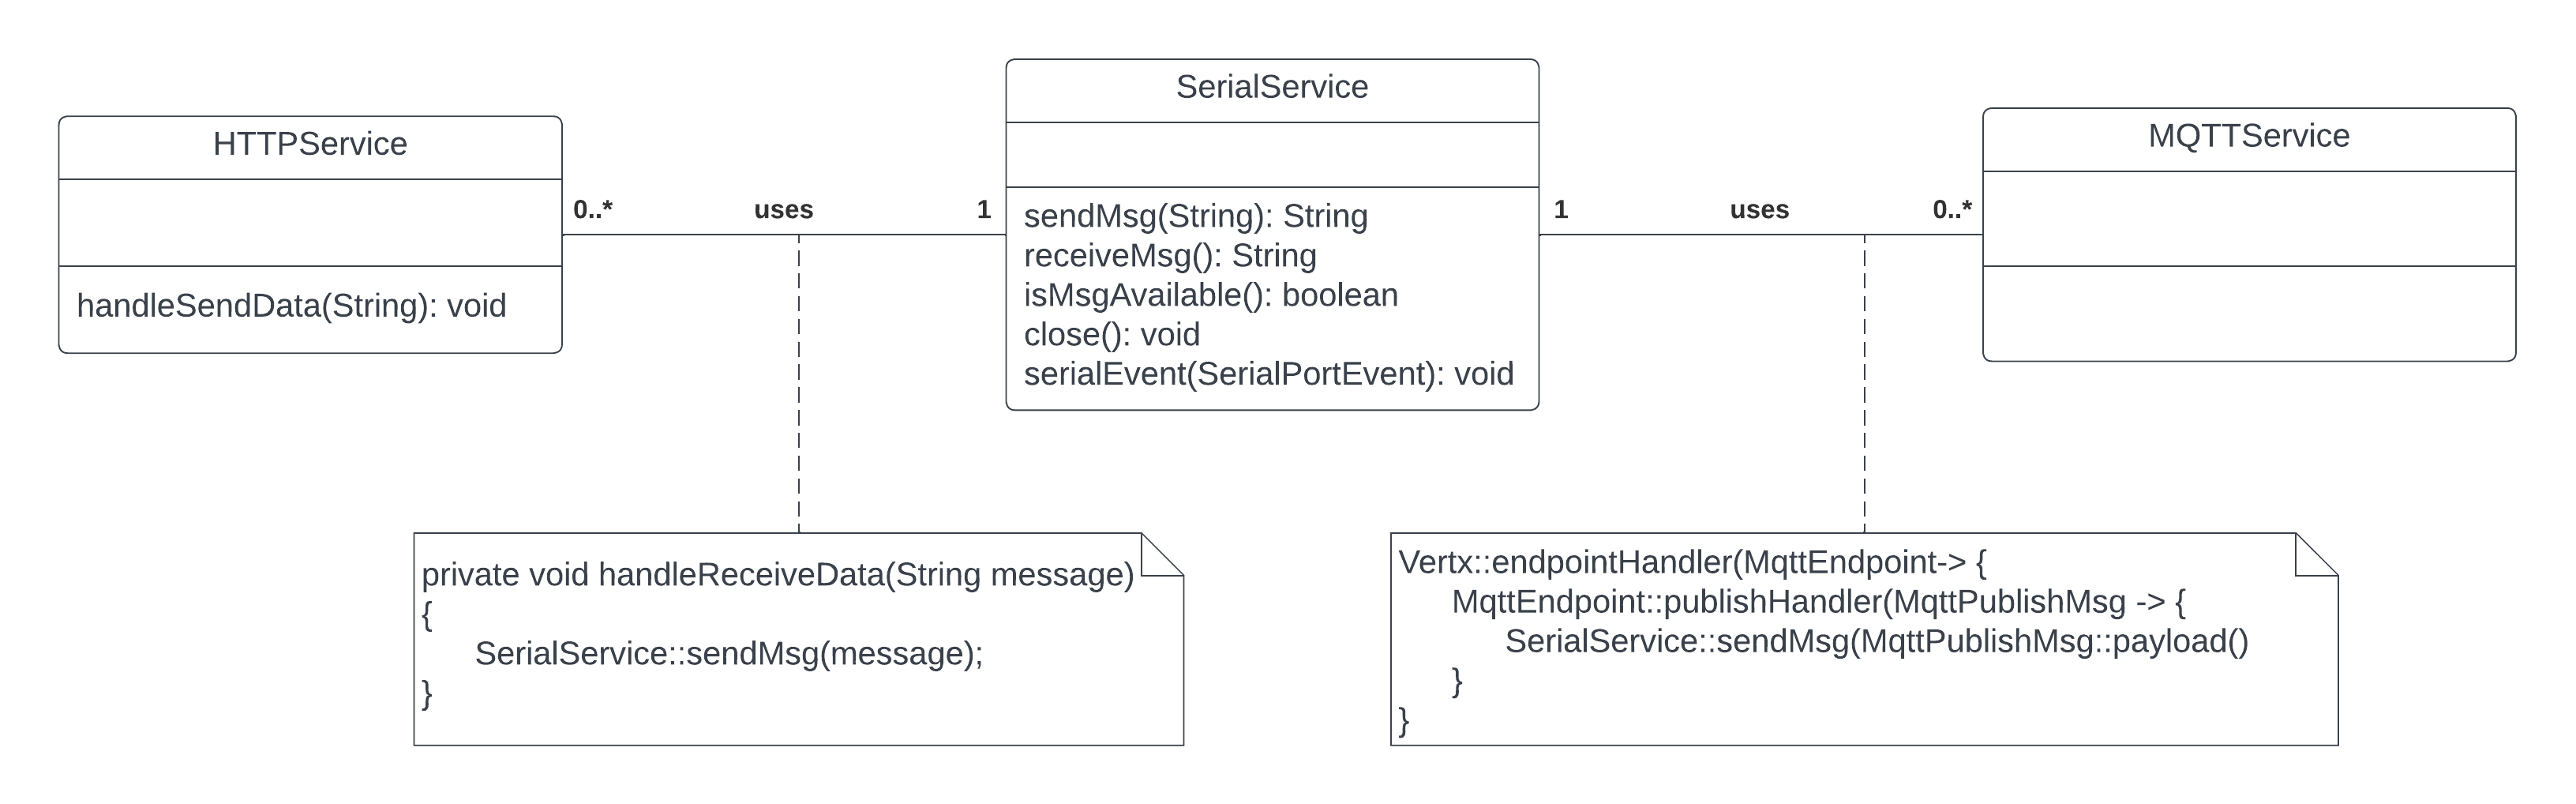
\includegraphics[width=\textwidth]{img/Classi - backend.png}
    \caption{Backend.}
    \label{fig:backend}
\end{figure}

Dove si può notare che il \texttt{SerialService} è un'istanza unica che viene condivisa fra tutti i servizi. Questo è stato fatto per evitare di aprire più canali di comunicazione seriale, che Arduino non supporta. Attraverso questo canale il server potrà indirizzare e ricevere dati da arduino. 

\subsection{Room Dashboard (Frontend)}
Dal punto di vista logico, per il lato frontend abbiamo suddiviso la logica in tre script JS: \texttt{charts.js}, \texttt{dashboard.js} e \texttt{socket.js}.
\begin{itemize}
    \item \texttt{charts.js} ha lo scopo di gestire la logica per l'aggiornamento dei due grafici. L'approccio adottato prevede il mettersi in ascolto sul webSocket \texttt{ws://localhost:8080}. Qualora il server avesse nuovi dati, lo script li può inviare su questo canale persistente e il client può riceverli. In questo modo si evita di dover effettuare richieste HTTP di overhead per richiedere i dati.
    \item \texttt{dashboard.js} gestisce l'invio dei dati per il controllo manuale della luce e della tenda. È necessario comunicare al server (che a sua volta informerà Arduino), l'istante in cui la pagina HTML prende il controllo dei sistemi, e il momento in cui si interrompe tale controllo. A tal proposito il nostro protocollo prevede l'invio di due tipi di messaggi.
    Il primo è questo
    \begin{lstlisting}[style=json]
    {
      "name": "manual_light/manual_roll",
      "measure": 0/1,
    }
    \end{lstlisting}
    Questo pacchetto rappresenta una configurazione iniziale. Notifica al server che è stato preso il controllo manualmente (1) o è stato disattivato (0) per uno dei due dispositivi.
    Il secondo è questo
    \begin{lstlisting}[style=json]
    {
      "name": "light/roll",
      "measure": 0..100,
    }
    \end{lstlisting}
    che indica che il dispositivo dev'essere acceso (1) o spento (0) nel caso della luce o in un range fra 0 e 100 per la tenda. Il meccanismo di invio è il medesimo della ricezione, i messaggi vengono inoltrati sullo stesso socket.
    \item \texttt{socket.js} si occupa di gestire la connessione con il server. In particolare, si occupa di gestire gli eventi di connessione e disconnessione, e di inviare i messaggi al server.
\end{itemize}
\subsection{Room Controller (Aruino)}
In questa sezione, come nel caso dell'ESP, poiché sia la luce che la tenda devono inviare e ricevere messaggi in formato JSON, abbiamo un'interfaccia \texttt{JSONSensor} che viene implementata da \texttt{Light} e \texttt{Roll}.
Tutta l'architettura è basata su una classe chiamata \texttt{MsgService} che mediante pattern Observer (il codice è stato ripreso dal task2 dal momento che era stato fatto quanto più possibile generico in modo da adattarsi a qualsiasi situazione), indirizza i pacchetti agli opportuni elementi. In particolare \texttt{MsgService} si occupa sia di ricevere i messaggi dal server (sia quelli provenienti dall'ESP che dalla dashboard), e indirizzarli a luce e tenda, le quali al loro interno avranno incapsulata la logica con cui adattarsi a questo tipo di messaggi, che indirizzare i messaggi generati da questi sensori verso il server. Oltre a questo, si occupa anche di gestire la logica del Bluetooth che, essendo basata anch'essa sulla seriale, è stata collassata all'interno della classe \texttt{MsgService}.
Tutto lo scambio di messaggi avviene sottoforma di istanze della classe \texttt{Msg} che incapsula la logica con cui i messaggi in formato JSON vengono deserializzati affinché si possa accedere ai vari campi. 

Di seguito è riportata la struttura del sottosistema 
\begin{figure}[H]
    \centering
    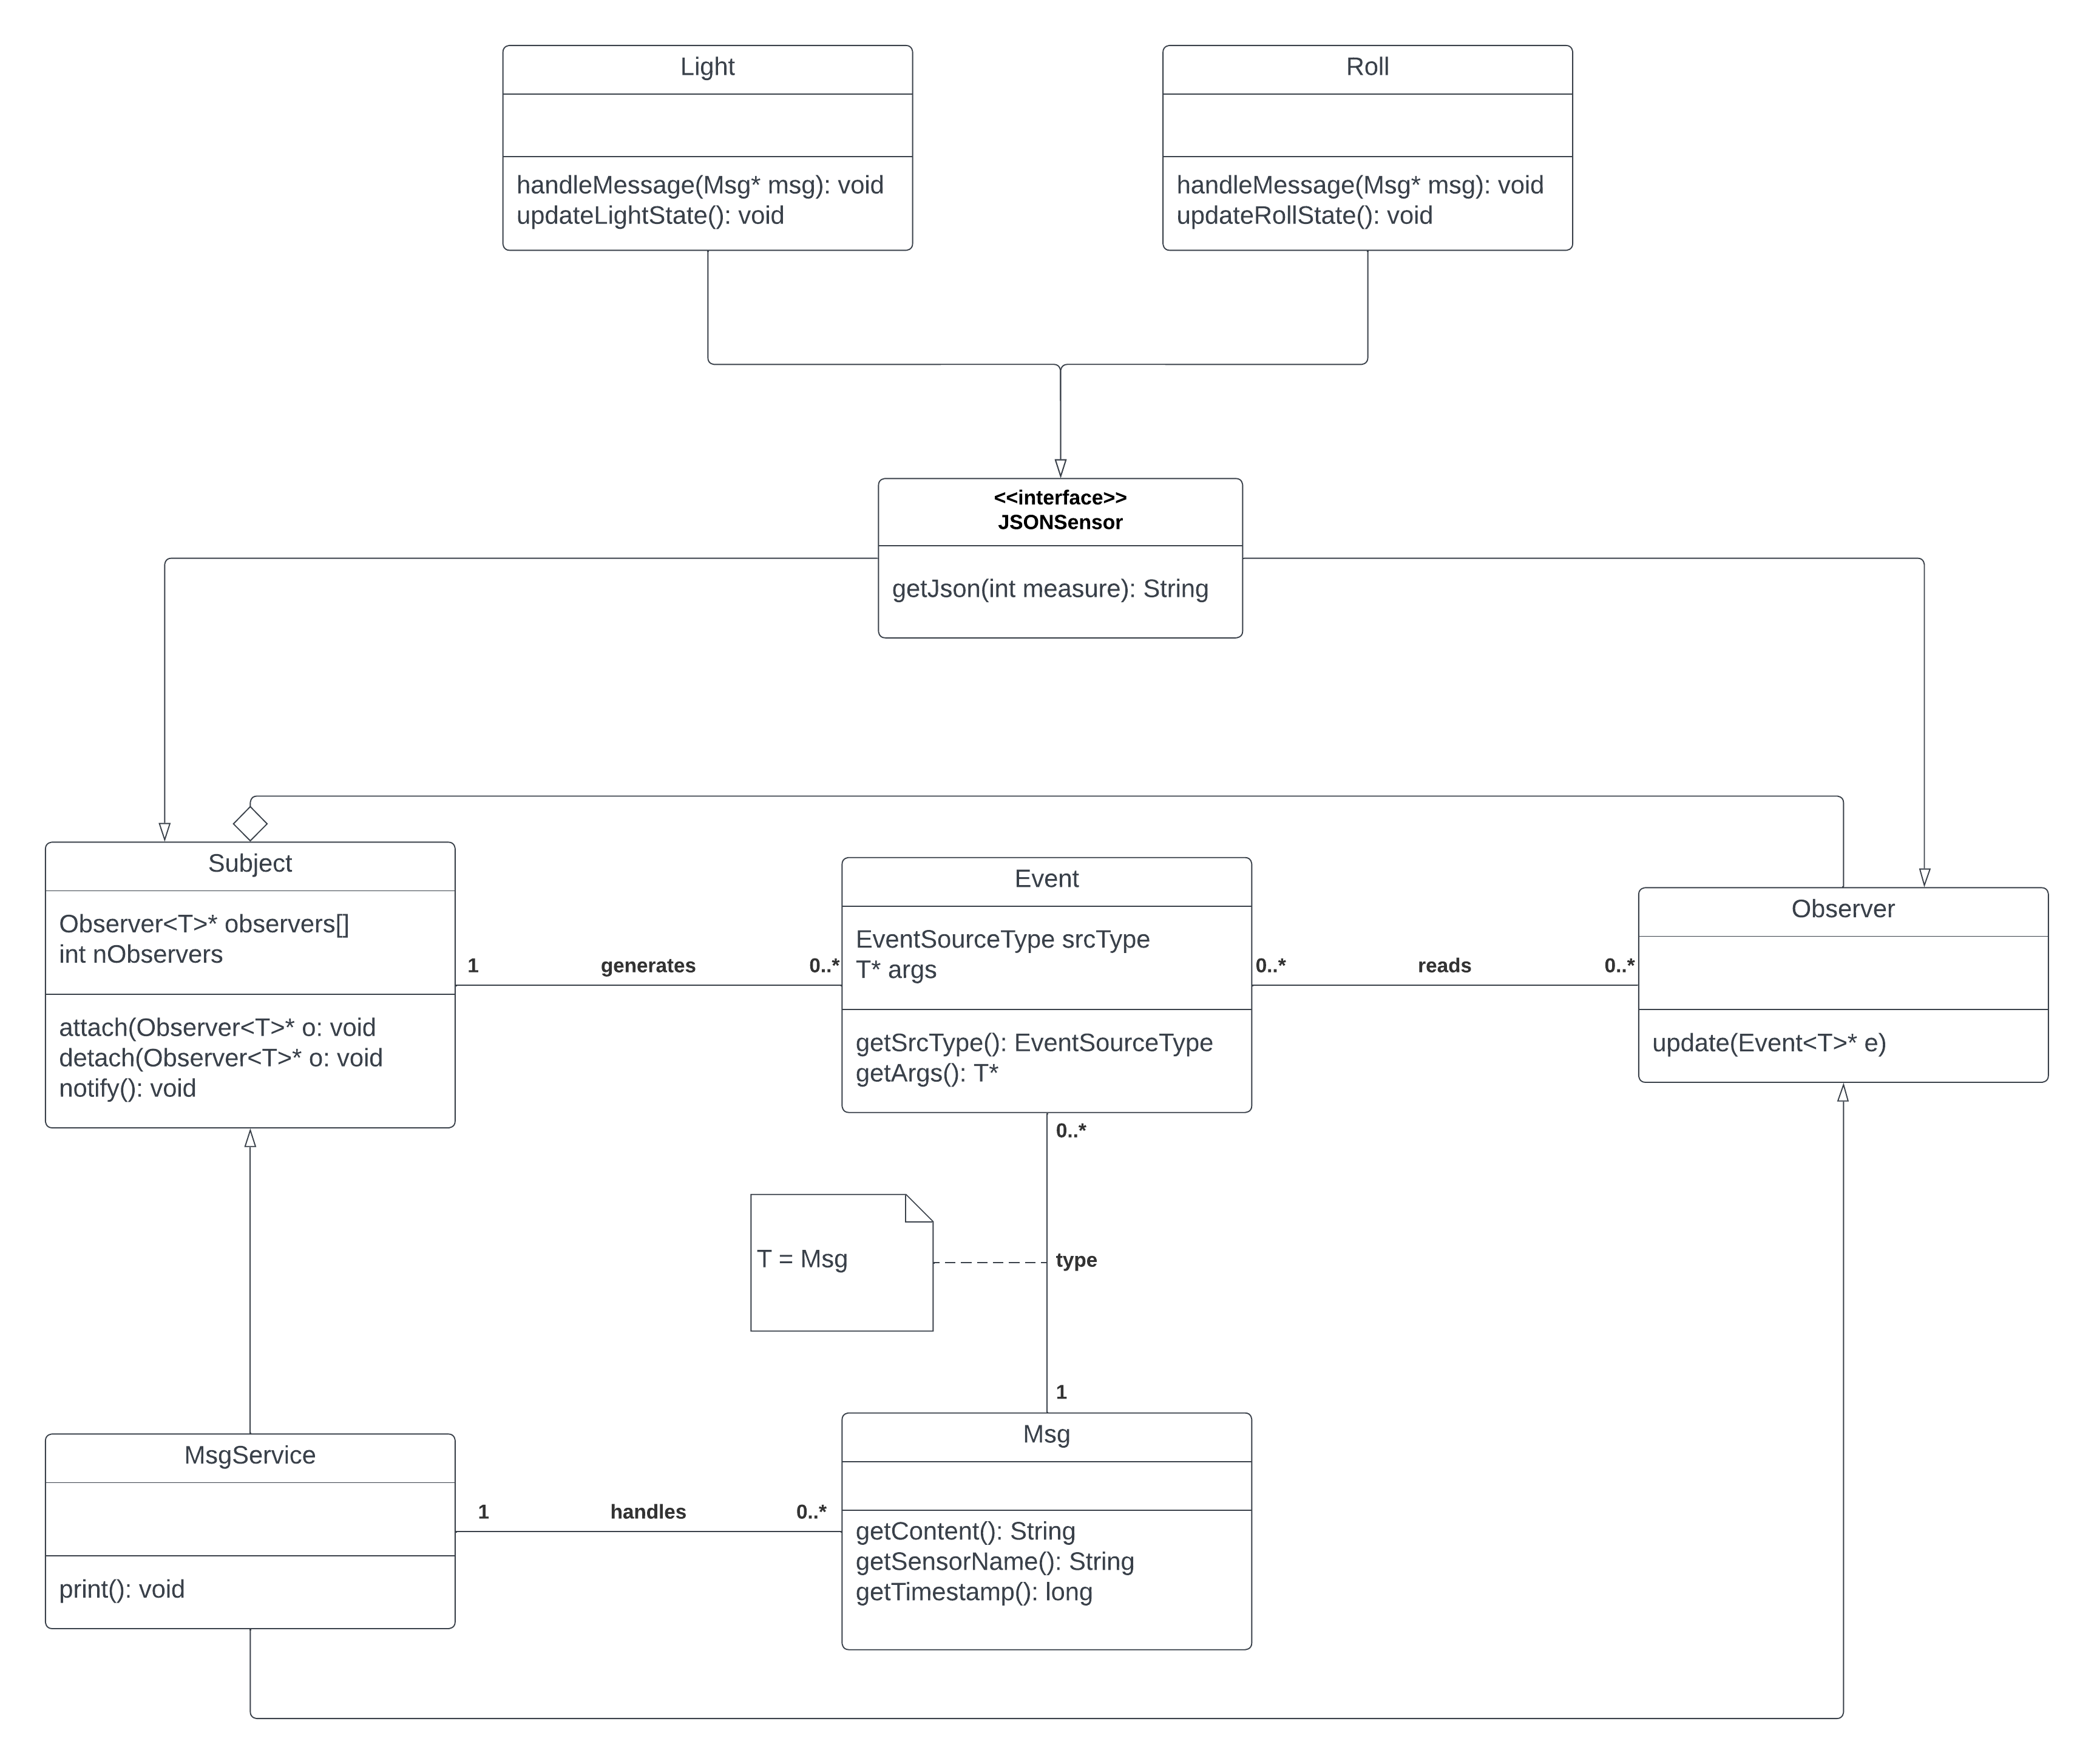
\includegraphics[width=0.9\textwidth]{img/Classi - arduino.png}
    \caption{Arduino.}
    \label{fig:arduino}
\end{figure}

\subsection{Room Mobile App (Android)}
L'app android sviluppata per il progetto si suddivide in due \emph{activity} (ciascuna rappresenta una schermata dell'applicazione).
\begin{enumerate}
    \item \texttt{Scan Activity}. È la prima schermata che appare all'utente all'avvio dell'applicazione. Serve per ricercare nuovi dispositivi bluetooth a cui connettersi.
    \item \texttt{Controller Activity}. Una volta avviata la connessione, l'interfaccia si aggiorna presentando questa activity che ha il compito di consentire all'utente il controllo di tenda e luci. Nello specifico si occupa di
    \begin{itemize}
        \item Inviare e ricevere dati da Arduino tramite bluetooth.
        \item Aggiornare di conseguenza la UI sulla base delle informazioni ottenute.
    \end{itemize}
\end{enumerate}
Per la lettura dei messaggi da parte di Arduino è stato creato un thread interno che, a partire da un \texttt{BluetoothSocket}, apre una input stream sulla quale si mette in ascolto. 
Per l'invio di messaggi ad Arduino esiste un'ulteriore thread che, sempre a partire dal socket \texttt{BluetoothSocket}, crea uno stream sul quale invia dati in formato JSON.
Tutte le modifiche effettuate sulla parte grafica vengono eseguite sul thread predefinito messo a disposizione da Android, chiamato \texttt{UiThread}.
Esiste poi un thread a parte \texttt{BluetoothClientConnectionThread} che si occupa di mantenere attiva la connessione fra client (il dispositivo) e Android.


\section{UI}
Per ovvie ragioni verranno di seguito mostrate solo le UI dell'applicazione web (dashboard) e dell'applicazione mobile.
Le UI sono state sviluppate in maniera tale da essere il più possibile intuitive e semplici da utilizzare.
\subsection{Room Dashboard (Frontend)}
Abbiamo utilizzato \texttt{Bootstrap} per lo sviluppo dell'interfaccia grafica e \texttt{Plotly}
per la rappresentazione dei grafici.
Le motivazioni per cui abbiamo scelto queste tecnologie sono le seguenti:
\begin{itemize}
    \item \texttt{Bootstrap} è un framework CSS che permette di sviluppare interfacce grafiche responsive e moderne. Inoltre, essendo molto diffuso, è facile trovare documentazione e risorse online.
    \item \texttt{Plotly.js} è una libreria JavaScript che permette di creare grafici interattivi. È stata scelta perché permette di creare grafici di qualità e perché è compatibile con \texttt{Bootstrap}. Inoltre è estremamente semplice da utilizzare e offre molta personalizzazione.
\end{itemize}
Di seguito è riportata un'immagine dell'interfaccia grafica.

\begin{figure}[H]
    \centering
    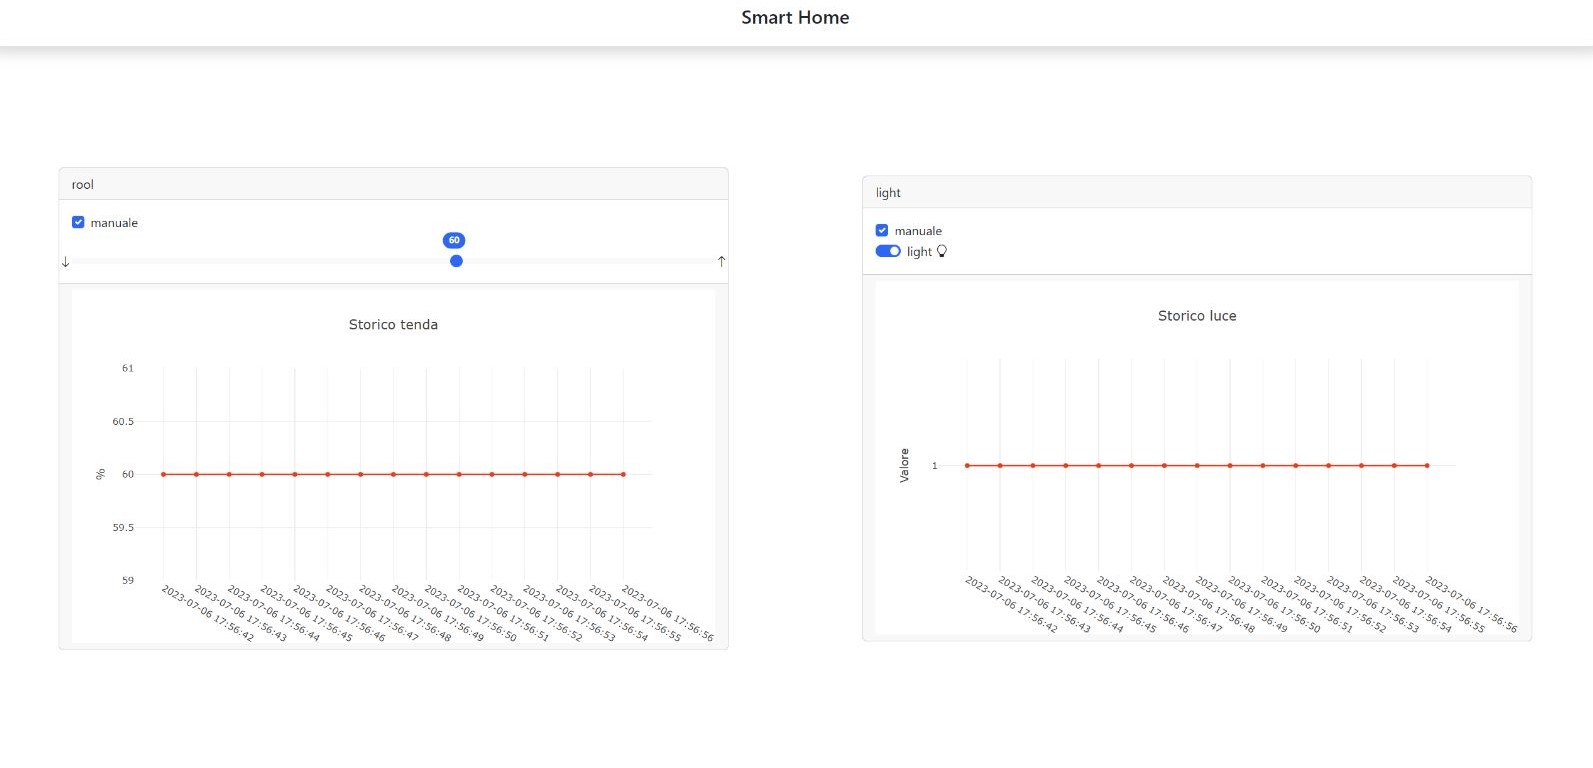
\includegraphics[width=0.9\textwidth]{img/Ui - dashboard.jpeg}
    \caption{Dashboard.}
    \label{fig:dashboard}
\end{figure}

\subsection{Room Mobile App (Android)}
L'app android è sviluppata, come già detto, in due \emph{activity}
\begin{itemize}
    \item \texttt{Scan Activity}. È la prima schermata che appare all'utente all'avvio dell'applicazione. Serve per ricercare nuovi dispositivi bluetooth a cui connettersi.
    \begin{figure}[H]
        \centering
        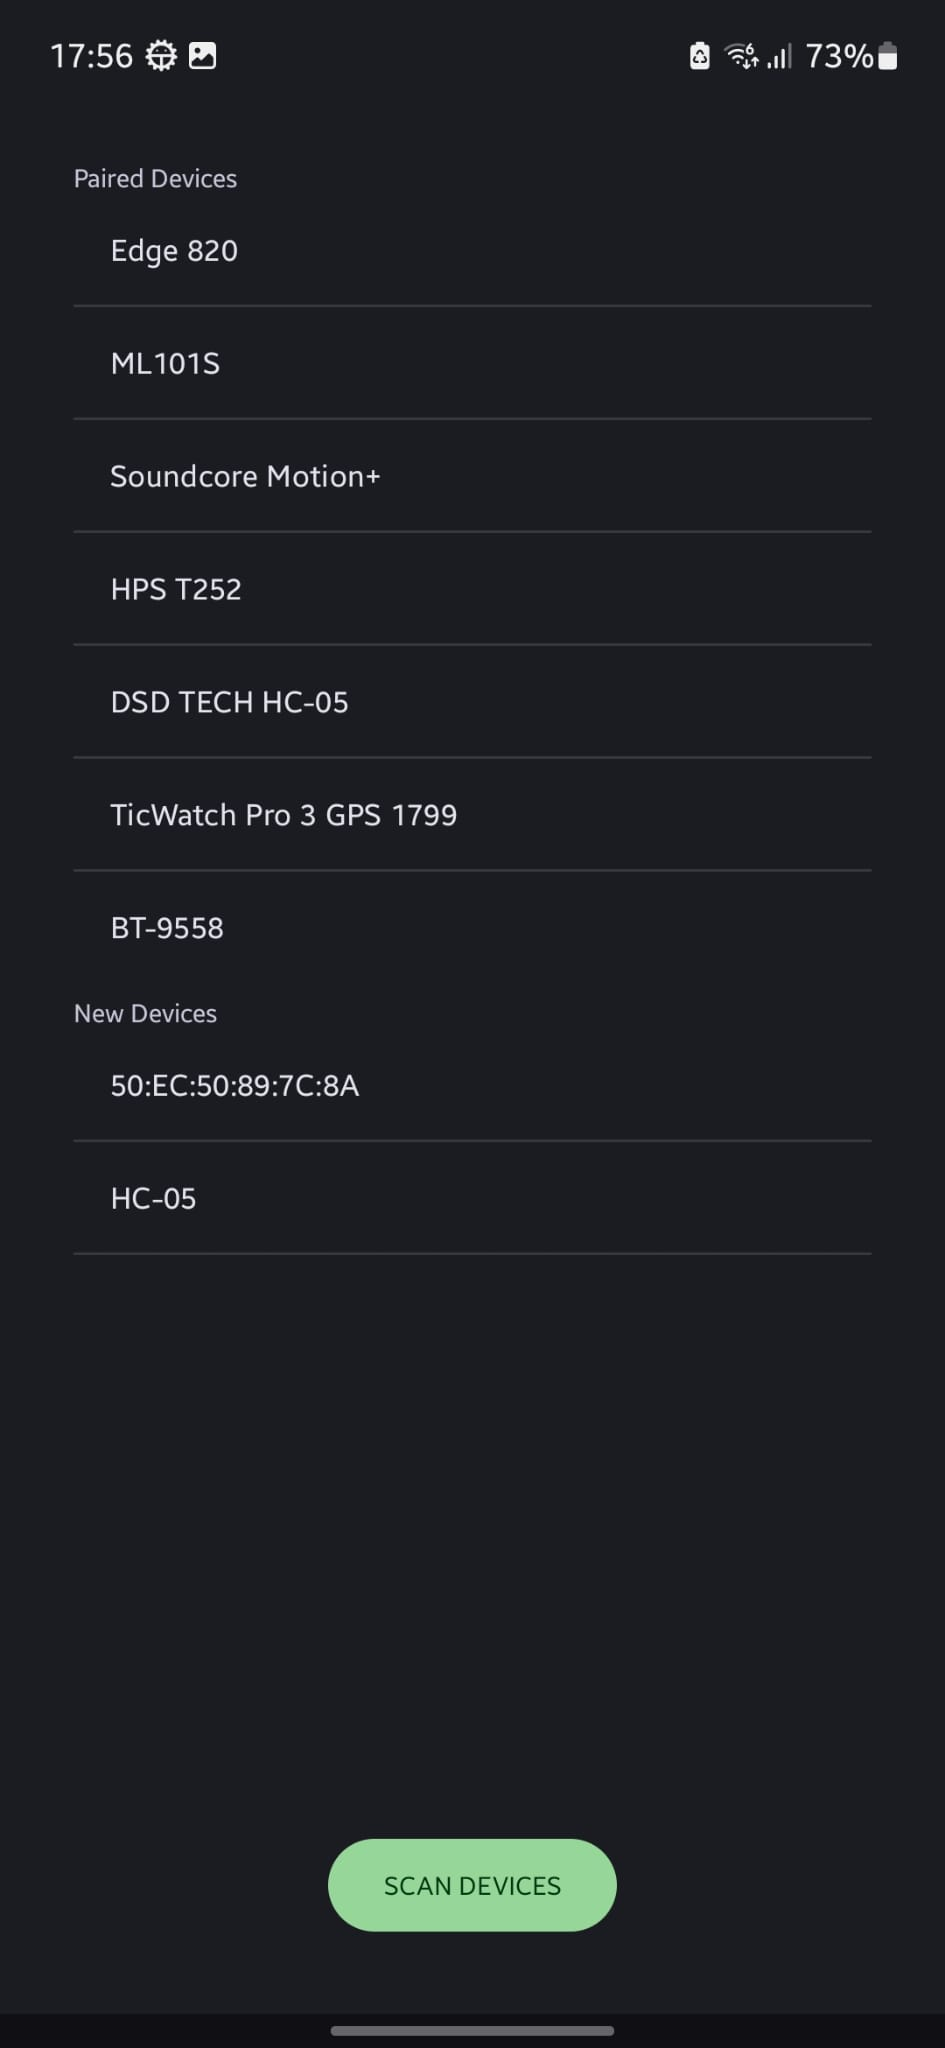
\includegraphics[width=0.4\textwidth]{img/Ui - scan.jpeg}
        \caption{Scan Activity.}
        \label{fig:scan}
    \end{figure}
    \item \texttt{Controller Activity}. Una volta avviata la connessione, l'interfaccia si aggiorna presentando questa activity che ha il compito di consentire all'utente il controllo di tenda e luci.
    \begin{figure}[H]
        \centering
        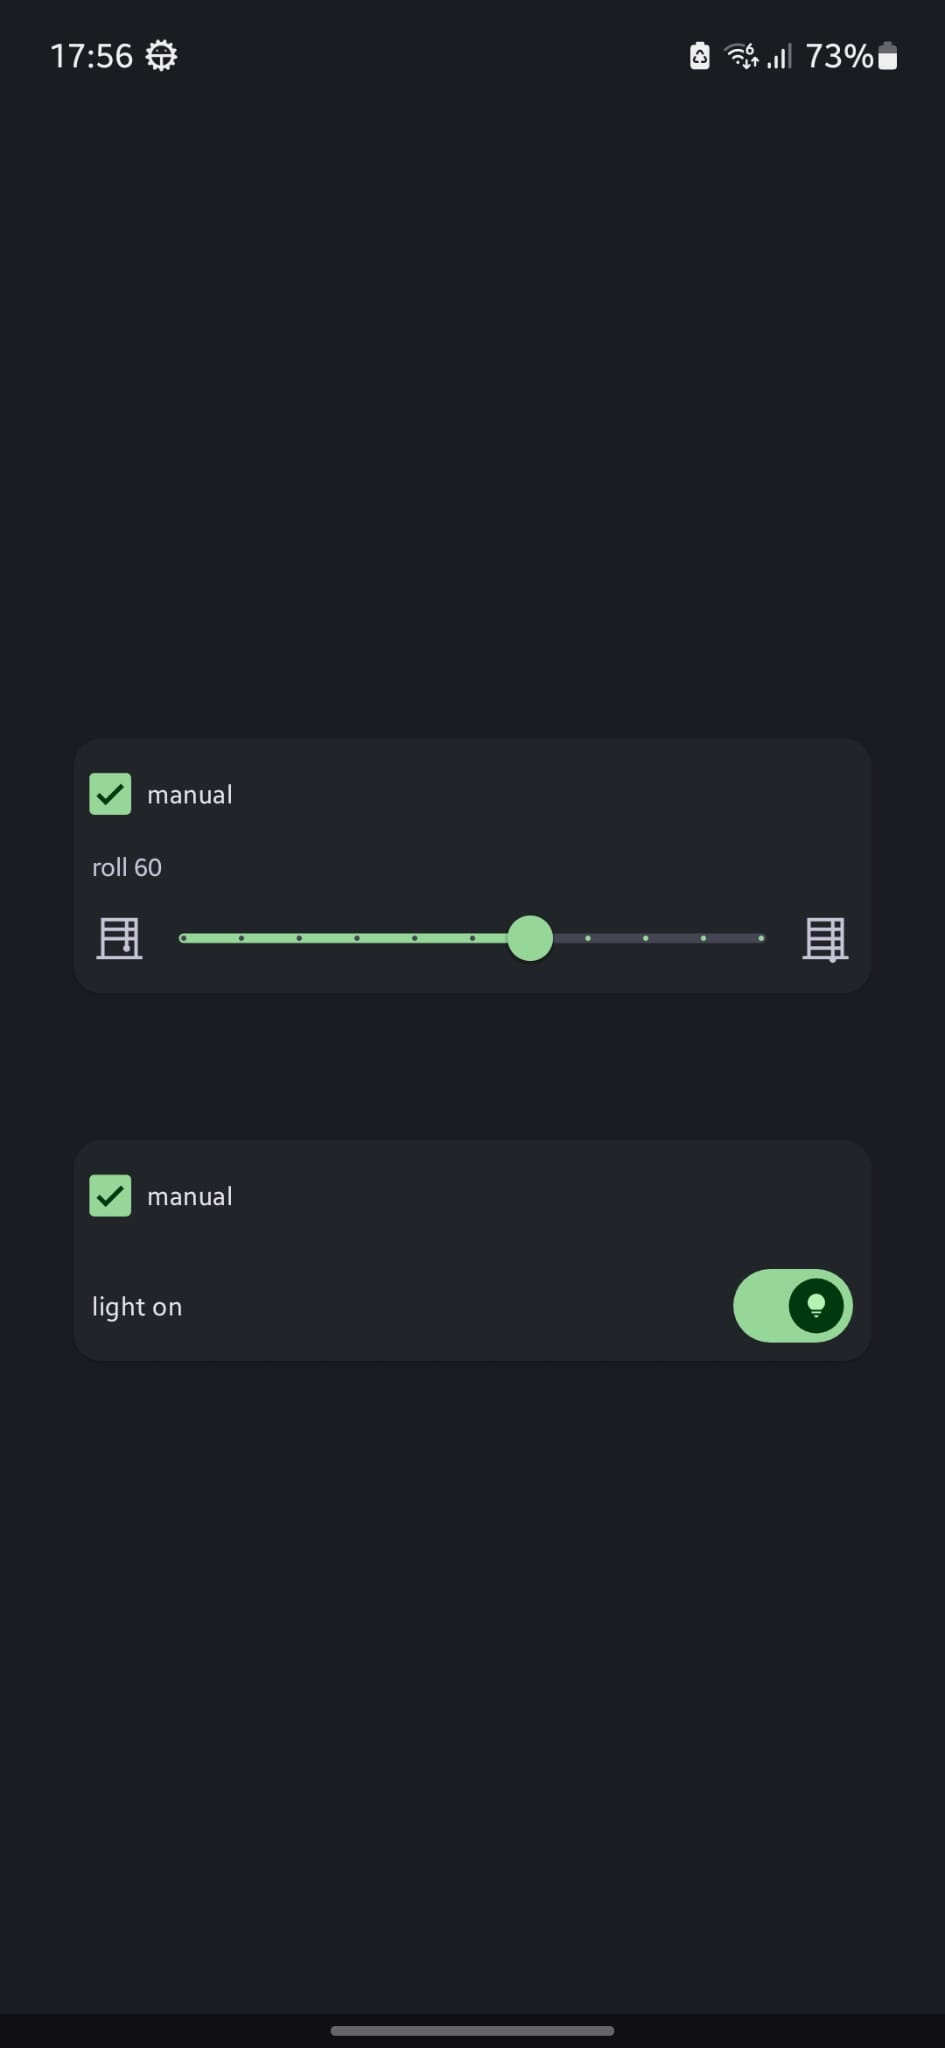
\includegraphics[width=0.4\textwidth]{img/Ui - controller.jpeg}
        \caption{Controller Activity.}
        \label{fig:controller}
    \end{figure}
\end{itemize}
Per entrambe è stato utilizzato il framework \texttt{Material Design V3} che permette di sviluppare interfacce grafiche moderne e intuitive. 




\chapter{Wirings}
In questo capitolo viene mostrata la rappresentazione del cablaggio.
Ovviamente sono mostrati separatamente i cablaggi di Arduino da quelli di ESP32.
\section{Descrizione Arduino}
Di seguito sono riportati i cablaggi per Arduino

\begin{figure}[H]
\centering
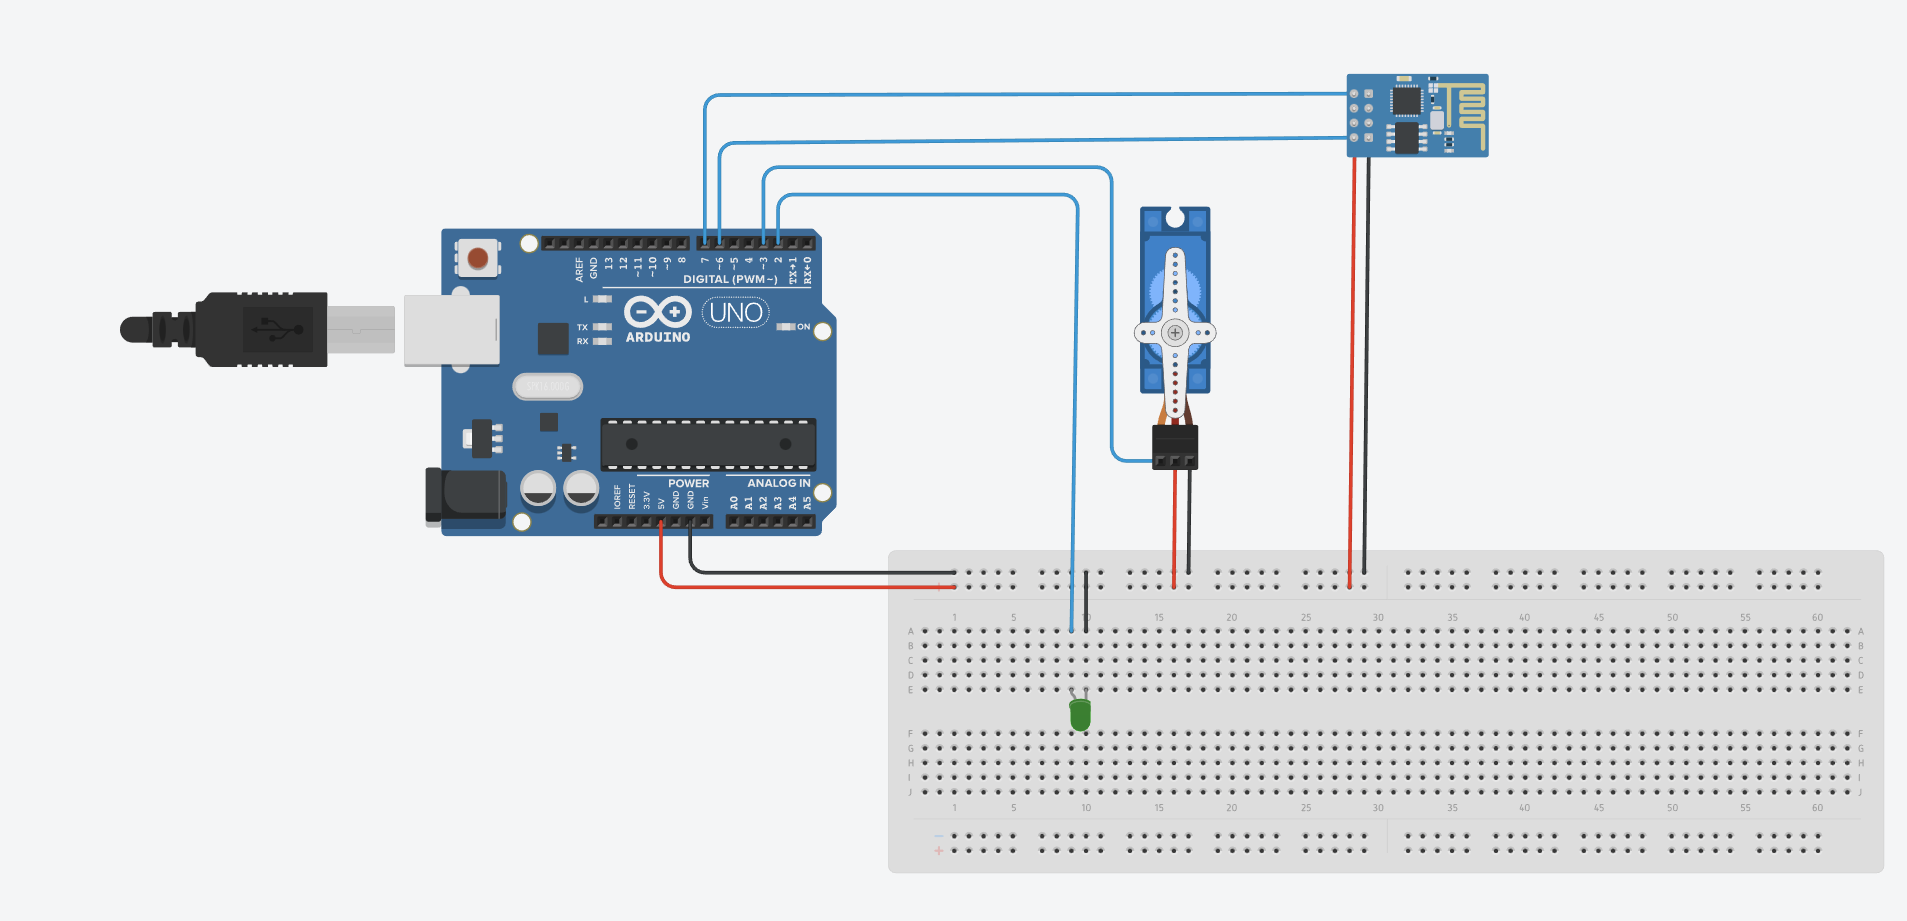
\includegraphics[width=\textwidth]{img/wire-arduino.png}
\caption{Schema del cablaggio di Arduino.}
\label{fig:wiringsarduino}
\end{figure}

Nell'immagine vediamo un led collegato al pin 2 (rappresenta la luce), un servo motore collegato al pin e (tenda) e infine un modulo bluetooth (poiché Thinkercad non disponeva del modulo bluetooth lo abbiamo sostituito con un modulo wifi, i cui pin restano però i medesimi), in particolare RX sul 6 e TX sul 7.

\section{Descrizione Esp32}
Poiché Thinkercad non mette a disposizione un modulo esp lo abbiamo sostituito nella figura che segue con un modulo bluetooth 

\begin{figure}[H]
\centering
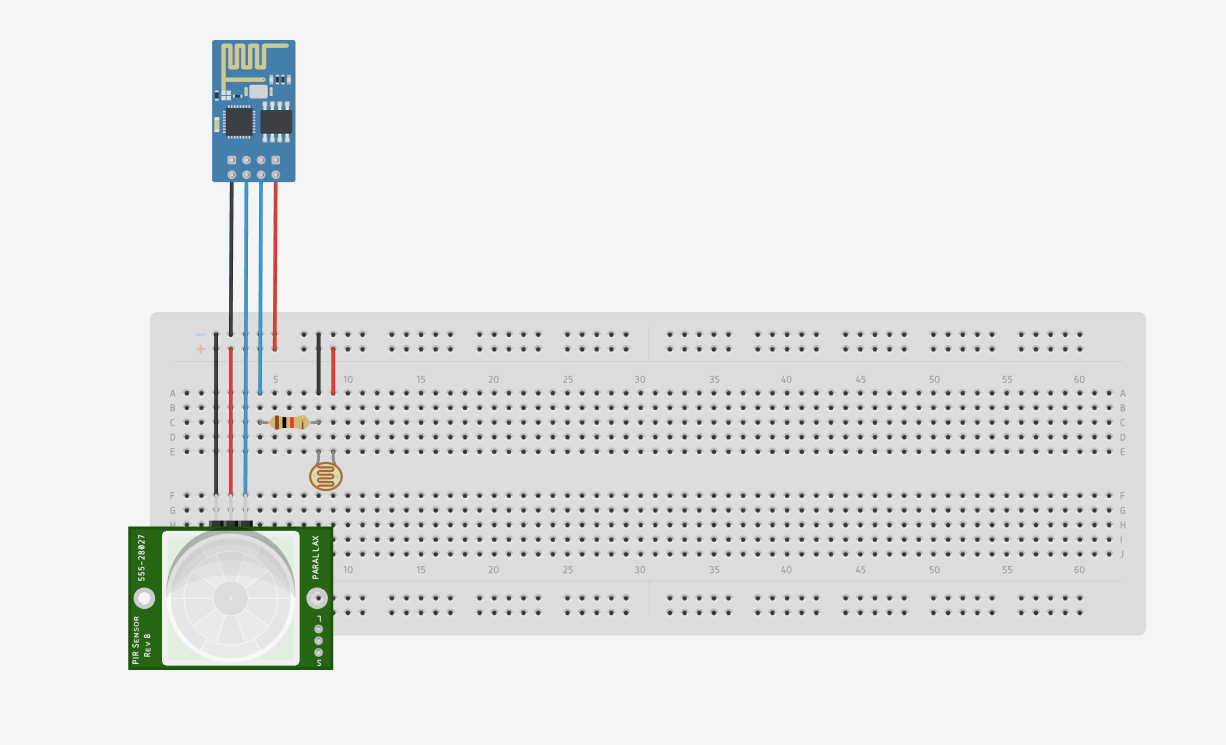
\includegraphics[width=\textwidth]{img/wire-esp.png}
\caption{Schema del cablaggio di Esp32.}
\label{fig:wiringsesp}
\end{figure}

Dall'immagine non si vede che la fotoresistenza è collegata al pin, mentre il pir a 

\end{document}